\documentclass[10pt,conference,compsocconf]{IEEEtran}

%\usepackage{times}
%\usepackage{balance}
\usepackage{url}
\usepackage{graphicx}	% For figure environment
\usepackage{tikz}
\usepackage{pgfplots}
\usetikzlibrary{calc,intersections,through,backgrounds, shapes}
\newcommand{\rfig}[1]{Figure~\ref{fig:#1}}


\begin{document}
\title{CIL Project: Collaborative Filtering}

\author{
	Dave Eschbach, Fanyi Zhou, Ulla Aeschbacher, Xiyue Shi\\
	Department of Computer Science, ETH Zurich, Switzerland
}

\maketitle

\begin{abstract}
 
\end{abstract}

\section{Introduction}

\section{Our Novel Solution}

\section{Comparing To Baselines}
We are comparing our novel solution to two others so that we can see how much improvement was done. The first of the two other solutions is the one from Assignment 3, where we were first completing the missing ratings in the matrix by setting them to the average over all observed ratings for a particular item. Then we tried to find an underlying structure in the data by performing SVD, where $X^{train} = UDV^T$. We vaired the number $k$ of eigenvalues used and truncated $U$ and $V$ accordingly. \rfig{rmse} shows the Root-Mean-Squared-Error for $k$ between 0 and 95, in intervals of 5. In \rfig{rmse_detail} we can see the error more clearly for $k$ between 5 and 95. Apparently, taking the biggest 10 eigenvalues is giving us the best approximation to the data structure. The best result we achieved on kaggle this way was 1.16473.

\begin{figure}[bp]
\centering
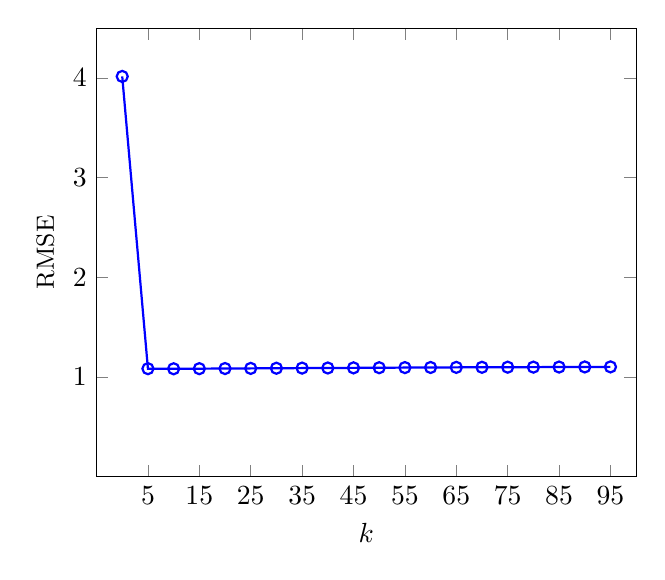
\begin{tikzpicture}
	\begin{axis}[
	xlabel={$k$},
	ylabel={\small{RMSE}},
	xmin=-5, xmax=100,
	ymin=0, ymax=4.5,
	xtick={5,15,25,35,45,55,65,75,85,95},
	ytick={1,2,3,4},
	x tick label style={color=black},
	legend style={
		draw=black,
		fill=white, 
		legend pos= north east,
		cells={anchor=west},},
	]
	\addplot[
		color=blue,
		mark=o,
		thick] 
		coordinates {(0,4.016120664688759)(5,1.0825649908614905)( 10,1.0815540472050764)(15,1.082655476468529)(20,1.084039420552301)(25, 1.08544809077967)(30,1.0870430839468697)(35,1.0883525165436614)(40,1.0894315213881094)(45,1.0906340685662301)(50,1.092158368755972)(55,1.0934254934023788)(60,1.0946167799674307)(65,1.0957557542153566)(70,1.096642058025502)(75,1.0975006311104656)(80,1.0980612147506275)(85,1.0989472280119372)(90,1.099854525492459)(95,1.1005504083912052)};
	\end{axis}
\end{tikzpicture}
\caption{RMSE in SVD with different $k$}
\label{fig:rmse}
\end{figure}

\begin{figure}[tbp]
\centering
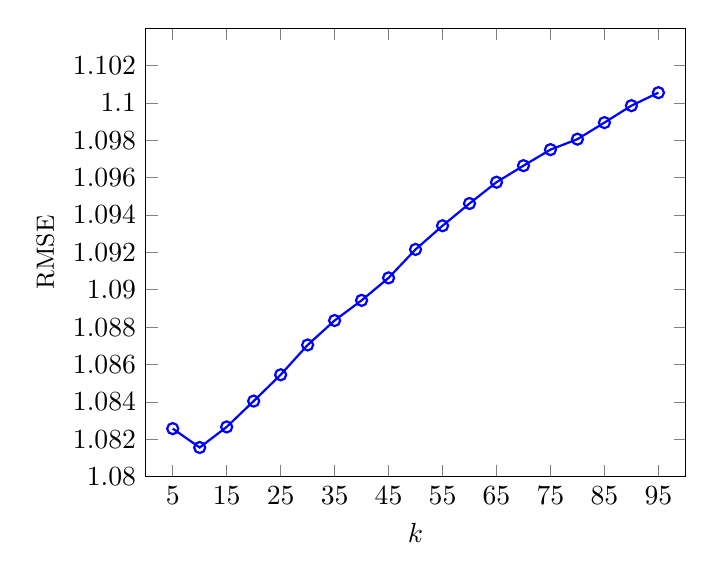
\begin{tikzpicture}
	\begin{axis}[
	xlabel={$k$},
	ylabel={\small{RMSE}},
	xmin=0, xmax=100,
	ymin=1.08, ymax=1.104,
	xtick={5,15,25,35,45,55,65,75,85,95},
	ytick={1.08,1.082,1.084,1.086,1.088,1.090,1.092,1.094,1.096,1.098,1.1,1.102},
	yticklabel style={/pgf/number format/.cd,fixed,precision=3},
	legend style={
		draw=black,
		fill=white, 
		legend pos= north east,
		cells={anchor=west},},
	]
	\addplot[
		color=blue,
		mark=o,
		thick] 
		coordinates {(5,1.0825649908614905)( 10,1.0815540472050764)(15,1.082655476468529)(20,1.084039420552301)(25, 1.08544809077967)(30,1.0870430839468697)(35,1.0883525165436614)(40,1.0894315213881094)(45,1.0906340685662301)(50,1.092158368755972)(55,1.0934254934023788)(60,1.0946167799674307)(65,1.0957557542153566)(70,1.096642058025502)(75,1.0975006311104656)(80,1.0980612147506275)(85,1.0989472280119372)(90,1.099854525492459)(95,1.1005504083912052)};
	\end{axis}
\end{tikzpicture}
\caption{RMSE in SVD with different $k$, shown in more detail}
\label{fig:rmse_detail}
\end{figure}

The second solution we are presenting here for comparison is a neural network. We trained a bidirectional LSTM. It has a bias layer, so that we could take into account that different people are rating higher or lower in general. We trid different dropout values, number of nodes, batch-sizes and trained over various epochs. In \rfig{lstm} you can see the Mean-Squared-Error loss over ten epochs of the neural network. The best result we achieved on kaggle this way was 1.04627. There are people that achieved much better results with a neural network \cite{tseng}, but our feeling is that our data was too sparse for this.

\begin{figure}[tbp]
\centering
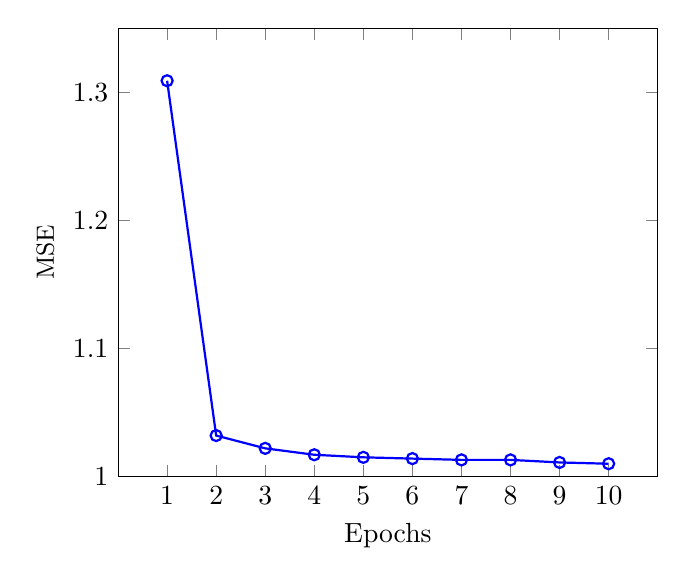
\begin{tikzpicture}
	\begin{axis}[
	xlabel={Epochs},
	ylabel={\small{MSE}},
	xmin=0, xmax=11,
	ymin=1.00, ymax=1.35,
	xtick={1,2,3,4,5,6,7,8,9,10},
	ytick={1.0,1.1,1.2,1.3},
	yticklabel style={/pgf/number format/.cd,fixed,precision=3},
	legend style={
		draw=black,
		fill=white, 
		legend pos= north east,
		cells={anchor=west},},
	]
	\addplot[
		color=blue,
		mark=o,
		thick] 
		coordinates {(1,1.309)(2,1.032)(3,1.022)(4,1.017)(5,1.015)(6,1.014)(7,1.013)(8,1.013)(9,1.011)(10,1.010)};
	\end{axis}
\end{tikzpicture}
\caption{MSE loss in LSTM over 10 epochs.}
\label{fig:lstm}
\end{figure}

Comparing the two solutions with our novel approach result of 0.98362 we can see

\section{Summary}

\newpage
\section{Computational Intelligence Laboratory Requirements}
\label{sec:cil}

Your semester project is a group effort. It consists of four parts:
\begin{enumerate}
\item The programming assignments you solve during the semester.
\item Developing a novel solution for one of the assignments, e.g. by
  combining methods from previous programming assignments into a novel
  solution.
\item Comparing your novel solution to previous assignments.
\item Writing up your findings in a short scientific paper.
\end{enumerate}

\subsection{Grading}

There are two different types of grading criteria applied to your
project, with the corresponding weights shown in brackets.
\begin{description}
\item[Competitive] \ \\
  The following criteria is scored based on your rank
  in comparison with the rest of the class.
  \begin{itemize}
  \item time taken for computation (10\%)
  \item average rank for all other criteria relevant to the task, for
    example reconstruction error and sparsity (20\%)
  \end{itemize}
  The ranks will then be converted on a linear scale into a grade
  between 4 and 6.
\item[Non-competitive] \ \\
  The following criteria is scored based on an
  evaluation by the teaching assistants.
  \begin{itemize}
  \item quality of paper (30\%)
  \item quality of implementation (20\%)
  \item creativity of solution (20\%)
  \end{itemize}
\end{description}

\subsection{Submission System}

The deadline for submitting your project report is Friday, 22 June
2012.
You need to submit:
\begin{itemize}
\item PDF of paper.
\item Archive (\texttt{.tar.gz} or \texttt{.zip}) of software. Please
  do not forget to include author information in the source archive.
\end{itemize}

\textbf{Important:} Please check the submission instructions on the webpage 
as it is the most updated instructions. 

\bibliographystyle{IEEEtran}
\bibliography{report}
\end{document}
